\documentclass[journal,12pt,twocolumn]{IEEEtran}
\usepackage{amsmath,amsfonts,amssymb,float,amsthm,gvv,listings,enumitem,mathtools}
\usepackage{graphicx}
\bibliographystyle{IEEEtran}
\vspace{3cm}
\title{NCERT Discrete}
\author{Pragnidhved Reddy\\EE23BTECH11050}
\date{}
\parindent 0px
\begin{document}
\maketitle
\newpage
\bigskip
\textbf{Question 10.5.2.8:}\\
An AP consists of $50$ terms of which $3^{rd}$ term is $12$ and the last term is $106$. Find the $29^{th}$ term.\\
\solution 
\begin{table}[H]
\centering
\begin{tabular}{|c|c|c|}\hline
\textbf{Parameter} & \textbf{Value} & \textbf{description}\\ \hline
$x(2)$ & $12$ & Third term\\ \hline
$x(49)$ & $106$ & Last term\\ \hline
$x(0)$ & $$ & First term \\ \hline
$d$ & $$ & Common difference\\ \hline
$x(n)$ & $(x(0)+nd)u(n)$ & general term \\ \hline
\end{tabular}
\caption{Input parameters}
\label{tab:table1}
\end{table}
\begin{align}
\label{eq:1}
x(2)&=x(0)+2d\\
\label{eq:2}
x(49)&=x(0)+49d
\end{align}
1) By solving \eqref{eq:1} and \eqref{eq:2} :
\begin{align}
\implies &d=2\\
\implies &x(0)=8
\end{align}
2) From the \tabref{tab:table1} :
\begin{align}
x(n)&=(x(0)+nd)u(n)\\
\implies x(n)&=(8+2n)u(n)
\end{align}
3) Finding $x(28)$ :
\begin{align}
x(28)&=x(0)+28(2)\\
\implies x(28)&=64
\end{align}
4) Finding the Z-transform :
\begin{align}
X(z)&=\sum_{k=-\infty}^{\infty}x(n) u(n) z^{-n}\\
&=\sum_{k=0}^{\infty}x(n) z^{-n}\\
\implies X(z)&=\frac{8-6z^{-1}}{(1-z^{-1})^2} \quad \text{ROC}\rightarrow(\abs{z}>1)
\end{align}
\begin{figure}[h!]
    \centering
    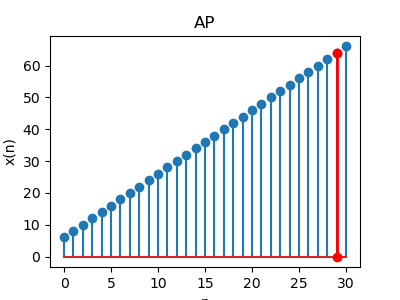
\includegraphics[width=\columnwidth]{figs/plot.png}
    \caption{graph of the given AP}
    \label{fig:1}
\end{figure}
\end{document}
